\documentclass{beamer}
\usepackage{tipa}
\usepackage{phonrule}
%\setbeamersize{text margin left=10pt,text margin right=10pt}
\usetheme{metropolis}
\usepackage{listings}
\usepackage{amsfonts}
\usepackage{dsfont}
\usepackage{amsmath}
\usepackage{bbm}
\usepackage{verbatim}
\usepackage{phonrule}
%\usepackage{tipa}
\usepackage{tikz}
\usetikzlibrary{fit}
\usepackage{color}
\usepackage{booktabs}
\usepackage{tipa}
\usepackage{amssymb}
\usepackage{verbatim}
\usepackage[absolute,overlay]{textpos}
\usepackage{pifont}% http://ctan.org/pkg/pifont
\usepackage{caption}
\usepackage{subcaption}
\newcommand{\cmark}{\ding{51}}%
\newcommand{\xmark}{\ding{55}}%
\usetikzlibrary{bayesnet}
\usetikzlibrary{decorations.markings}
\usetikzlibrary{decorations.pathmorphing}
\tikzset{squiggle/.style={decorate, decoration={snake,amplitude=.4mm}}}
\usepackage{xcolor}
\definecolor{pop1}{HTML}{1F78b4}
\definecolor{pop2}{HTML}{164C13}
\definecolor{pop3}{HTML}{d95F02}
\definecolor{orange}{HTML}{d95F02}
\definecolor{teal}{HTML}{1b9e77}
\newcommand{\pop}[1]{\textcolor{pop1}{#1}}
\newcommand{\popp}[1]{\textcolor{pop2}{#1}}
\newcommand{\tree}[1]{\textcolor{pop3}{#1}}
\newcommand{\orange}[1]{\textcolor{orange}{#1}}
\newcommand{\teal}[1]{\textcolor{teal}{#1}}
\newcommand{\code}[1]{{\footnotesize\texttt{#1}}}
\newcommand{\greenCode}[1]{{\footnotesize\popp{\code{#1}}}}
\newcommand{\blueCode}[1]{{\footnotesize\pop{\code{#1}}}}
\definecolor{backgroundGreen}{HTML}{23373b}
\lstset{escapeinside={<@}{@>}}
\usepackage{pgf}  

%% \usepackage[sfdefault]{FiraSans} %% option 'sfdefault' activates Fira Sans as the default text font
%% \usepackage[T1]{fontenc}
%% \renewcommand*\oldstylenums[1]{{\firaoldstyle #1}}


\newcommand{\Expect}{\mathds{E}} %{{\rm I\kern-.3em E}}
\newcommand{\1}[1]{\mathds{1}\left[#1\right]}
\newcommand{\E}{\mathds{E}} %{{\rm I\kern-.3em E}}
\newcommand{\indicator}{\mathds{1}} %{{\rm I\kern-.3em E}}
\newcommand{\expect}{\mathds{E}} %{{\rm I\kern-.3em E}}
\newcommand{\probability}{\mathds{P}} %{{\rm I\kern-.3em P}}
\DeclareMathOperator*{\argmin}{arg\,min} % thin space, limits underneath in displays
\DeclareMathOperator*{\argmax}{arg\,max} % thin space, limits underneath in displays
\DeclareMathOperator*{\argmaxk}{arg\,top-\textit{k}} % thin space, limits underneath in displays

\usepackage[absolute,overlay]{textpos}

\newcommand{\nextForm}[1]{\rotatebox[origin=c]{270}{$_{\curvearrowright}$}$_{#1}$}
 
\usepackage{amsfonts}
\usepackage{tabularx}
%\usepackage{color}
\usepackage{graphicx}
\usepackage{booktabs}
\usepackage{xcolor}
\usepackage{tikz}
\usetikzlibrary{trees}
\usetikzlibrary{fit}
\usetikzlibrary{calc}
\usetikzlibrary{bayesnet}
\usepackage[absolute,overlay]{textpos}
\usepackage{stmaryrd}
\newcommand{\sem}[1]{\llbracket #1\rrbracket}
\newcommand{\eval}[1]{\llbracket #1\rrbracket}
\newcommand{\tuple}[1]{\ensuremath{\left \langle #1\right \rangle}}
\newcommand{\messageOverlay}[1]{
      \tikz[overlay,remember picture]
      \node[align=left,fill=backgroundGreen,text=white] at (current page.center){#1};
}
\newcommand{\myPaper}[1]{
  \tikz[overlay,remember picture]
  \node[anchor=south west,align=left] at (current page.south west){#1};
}
\newcommand{\myPaperRight}[1]{
  \tikz[overlay,remember picture]
  \node[anchor=south east,align=left] at (current page.south east){#1};
}
\usepackage{booktabs}
\usepackage{tipa}
\usepackage{amssymb}
\usepackage{verbatim}
\usepackage[absolute,overlay]{textpos}
\usepackage{pifont}% http://ctan.org/pkg/pifont
%% \newcommand{\cmark}{\ding{51}}%
%% \newcommand{\xmark}{\ding{55}}%
\usetikzlibrary{bayesnet}
\usetikzlibrary{decorations.markings}

\newcommand\Wider[2][3em]{%
\makebox[\linewidth][c]{%
  \begin{minipage}{\dimexpr\textwidth+#1\relax}
  \raggedright#2
  \end{minipage}%
  }%
}
\definecolor{backgroundBeige}{RGB}{250,250,250}
\newcommand{\denotation}[1]{{\llbracket #1 \rrbracket}}

\usepackage[utf8]{inputenc}
\newcommand{\reduce}{\longrightarrow}
\usepackage{amssymb}% http://ctan.org/pkg/amssymb
\usepackage{pifont}% http://ctan.org/pkg/pifont

\usepackage{fancyvrb}

\usepackage[most]{tcolorbox}
\definecolor{block-gray}{gray}{0.10}
\newtcolorbox{mycode}{colback=block-gray,grow to right by=0mm,grow to left
by=0mm, boxrule=0pt,boxsep=0pt,breakable,fontupper=\color{white}}

%% Program ::=
%%   (if Bool List
%%     (append RecursiveList
%%             RecursiveList
%%             RecursiveList))
%% RecursiveList ::= List
%%          | (recurse List)

            

\usepackage{arydshln}

%\newcommand{\Expect}{\mathds{E}} %{{\rm I\kern-.3em E}}
\newcommand{\Probability}{\mathds{P}} %{{\rm I\kern-.3em P}}

%\DeclareMathOperator*{\argmax}{arg\,max}
%Information to be included in the title page:
\title{DreamCoder:\\Bootstrapping Inductive Program Synthesis with Wake-Sleep Library Learning}
\author{Kevin Ellis$^1$ Catherine Wong$^2$ Maxwell Nye$^2$ Mathias Sabl\'e-Meyer$^3$\\  Lucas Morales$^2$ Luke Hewitt$^2$ Luc Cary$^2$\\Armando Solar-Lezama$^2$ Joshua B. Tenenbaum$^2$}
\institute{PLDI. $^1$Cornell; $^2$MIT; $^3$PSL/Collège de France \& NeuroSpin}
\date{2021}
  
 
\begin{document}
 
\frame{\titlepage}

\begin{frame}{Inductive program synthesis}

  \textbf{Program synthesis:} automatically write computer programs from a specification of what they should do

  \pause

  \textbf{Inductive program synthesis:} Learning programs from examples

\end{frame}


\begin{frame}{}
  \Wider[5em]{  \begin{tabular}{cc}
      FlashFill (Gulwani 2012)&\\
      \begin{tabular}{c}
        \includegraphics[width = 6cm]{ff_example}
      \end{tabular}&
      \begin{tabular}{c}
        \visible<3->{\includegraphics[width = 5cm]{ff_DSL}}
      \end{tabular}\\
      \visible<2->{Szalinski (Nandi 2020)}&\\
      \begin{tabular}{c}
        \visible<2->{\includegraphics[width = 6cm]{uwCAD_example}}
      \end{tabular}&
      \begin{tabular}{c}
        \visible<3->{\includegraphics[width = 5cm]{uwCAD_DSL}}
      \end{tabular}
  \end{tabular}}
\end{frame}

%% \begin{frame}{Visual programs}
%%   \Wider[6em]{\centering\begin{tabular}{c}
%%     \includegraphics[width = 10cm]{tutorial/ns}\\{\small Mao$^*$, Zhang$^*$, et al 2019}\\
%%     \visible<1->{\includegraphics[width = 10cm]{assets/we_are_cool_4.png}}\\
%%     \visible<1->{{\small Ellis$^*$, Nye$^*$, Pu$^*$, Sosa$^*$, et al 2019}}\\
%%     %% \includegraphics[width = 10cm]{graphicsTeaser1}\\
%%     %% Ellis, Ritchie, et al 2018\\\\
%%     \begin{tabular}{cc}
%%       \visible<1->{\includegraphics[width = 5cm]{tutorial/kind}}&
%%       \visible<1->{\includegraphics[width = 8cm]{tutorial/shape2}}
%%       \\
%%       \visible<1->{\small Young et al 2019}&\visible<1->{\small Tian et al 2019}
%%       \end{tabular}
%%   \end{tabular}}
%%   %% \begin{tikzpicture}
%%   %%   \node[draw,label={hand drawing}](picture1) at (0,-1) {\includegraphics[height = 2.2cm]{TikZfigures/expert-31-trim.png}};
%%   %%   \node[label={%% [align=right]left:
%%   %%       machine-generated program},draw,right=1cm of picture1] (c1) {
%%   %%     \begin{lstlisting}[basicstyle = \small\ttfamily]
%%   %%       for (0 <= i < 3)
%%   %%       rectangle(3*i,-2*i+4,
%%   %%       3*i+2,6)
%%   %%       for (0 <= j < i + 1)
%%   %%       circle(3*i+1,-2*j+5)
%%   %%     \end{lstlisting}
%%   %%   };
    
%%   %%   \draw[very thick,->] (picture1.east)  -- (c1.west);

%%   %%   %    \node(l1)[anchor=south] at ([yshift=0.75cm,xshift=2.5cm]picture1.north) {model infers program from drawing};
%%   %% \end{tikzpicture}  
%% \end{frame}
%% \begin{frame}{Where does this language come from?}
%%   \Wider[6em]{\centering\begin{tabular}{c}
%%     \includegraphics[width = 10cm]{tutorial/nsl}\\{\small Mao$^*$, Zhang$^*$, et al 2019}\\
%%     \visible<1->{\includegraphics[width = 10cm]{assets/we_are_cool_4l.png}}\\
%%     \visible<1->{{\small Ellis$^*$, Nye$^*$, Pu$^*$, Sosa$^*$, et al 2019}}\\
%%     %% \includegraphics[width = 10cm]{graphicsTeaser1}\\
%%     %% Ellis, Ritchie, et al 2018\\\\
%%     \begin{tabular}{cc}
%%       \visible<1->{\includegraphics[width = 5cm]{tutorial/kindl}}&
%%       \visible<1->{\includegraphics[width = 8cm]{tutorial/shape2l}}
%%       \\
%%       \visible<1->{\small Young et al 2019}&\visible<1->{\small Tian et al 2019}
%%       \end{tabular}
%%   \end{tabular}}
%% \end{frame}

%% \begin{frame}{Human-level Program induction}
%%   \begin{tikzpicture}
%%     \node at(0,0) {\includegraphics[width = 8cm]{../ecPaper/characters.png}};
%%     \node at(-3,2) {\includegraphics[width = 8cm]{../ecPaper/Brendan.jpg}};

%%     \node at (-5,-4) {  Lake et al 2015};
%%     \end{tikzpicture}
%% \end{frame}




\begin{frame}{Learning to write code} %Growing domain-specific knowledge}
  
  %  \Large
  Goal: acquire domain-specific knowledge needed to induce a class of programs


  
  \vspace{0.75cm}

  \Wider[4em]{
    \begin{itemize}
    \item Library of abstractions (domain specific language) \\ %; generative model over programs)
      \item      Inference strategy (synthesis algorithm)
      \end{itemize}
  }
  
  \vspace{0.75cm}
  
  %% \visible<2>{
  %% \begin{tikzpicture}
  %%   \node(problem) at (0,0) {\includegraphics[width = 2cm]{figures/cubic.png}};
  %%   \node(synthesizer)[draw,align=center] at ([xshift=3cm]problem.east) {Learned \\program inducer};
  %%   \draw[->] (problem.east) -- (synthesizer.west);
  %%   \node(program)[draw, align=center] at ([xshift=3cm]synthesizer.east) {program:\\$f(x) = 0.3x^3+$\\$1.1x^2-2x+0.6$};
  %%   \draw[->] (synthesizer.east) -- (program.west);
  %% \end{tikzpicture}
  
  %%   \vspace{0.2cm}Concepts: $x^3$, $\alpha x + \beta$, etc\\Inference strategy: neurosymbolic search for programs}
  %% \renewcommand\code\texttt
  %%   \only<3>{
  %% \begin{tikzpicture}
  %%   \node(problem) at (0,0) {\includegraphics[width = 2cm]{figures/radialCircle.png}};
  %%   \node(synthesizer)[draw,align=center] at ([xshift=3cm]problem.east) {Learned \\program inducer};
  %%   \draw[->] (problem.east) -- (synthesizer.west);
  %%   \node(program)[draw, align=center] at ([xshift=3cm]synthesizer.east) {program:\\\code{(radial-symmetry 5}\\\code{ (circle 3))}};
  %%   \draw[->] (synthesizer.east) -- (program.west);
  %% \end{tikzpicture}
  
  %% \vspace{0.2cm}Concepts: \code{circle}, \code{radial-symmetry}, etc\\Inference strategy: neurosymbolic search for programs
  %%   }
\end{frame}


\begin{frame}{Library learning}
  \Wider[5em]{
    \begin{center}
      \begin{tabular}{cc}
        \includegraphics[height=\textheight]{figures/figureOneFinal1_primitives}&
        \includegraphics[height=\textheight]{figures/figureOneFinal1_problem}
      \end{tabular}
    \end{center}
  }
\end{frame}

\begin{frame}[t]{Library learning}
\Wider[5em]{  \begin{center}
    \begin{tabular}{ccc}
      \includegraphics[height=0.6\textheight]{figures/figureOneFinal1_primitives}&
      \phantom{testingtesting}&
      \includegraphics[height=0.6\textheight]{figures/figureOneFinal1_problem}
    \end{tabular}
\end{center}}
\end{frame}


\begin{frame}{Library learning}
%  \centering
  
  \only<1>{  \Wider[5em]{\includegraphics[width = \textwidth]{figures/figureOneFinal1}}}
  \only<2>{  \Wider[5em]{\includegraphics[width = \textwidth]{figures/figureOneFinal2_layer1}}}
  \only<3>{  \Wider[5em]{\includegraphics[width = \textwidth]{figures/figureOneFinal2_layer1_exploded}}}
  \only<4>{  \Wider[5em]{\includegraphics[width = \textwidth]{figures/figureOneFinal2_layer1}}}
  \only<5>{  \Wider[5em]{\includegraphics[width = \textwidth]{figures/figureOneFinal2_layer2}}}
  \only<6>{  \Wider[5em]{\includegraphics[width = \textwidth]{figures/figureOneFinal2_layer2_exploded}}}
  \only<7>{  \Wider[5em]{\includegraphics[width = \textwidth]{figures/figureOneFinal2_layer2}}}
  \only<8>{  \Wider[5em]{\includegraphics[width = \textwidth]{figures/figureOneFinal2}}}
  \only<9>{  \Wider[5em]{\includegraphics[width = \textwidth]{figures/figureOneFinal2_exploded}}}
  \only<10>{  \Wider[5em]{\includegraphics[width = \textwidth]{figures/figureOneFinal3}}}
  \only<11>{  \Wider[5em]{\includegraphics[width = \textwidth]{figures/figureOneFinal3_explained_exploded}}}
  \only<12->{  \Wider[5em]{\includegraphics[width = \textwidth]{figures/figureOneFinal3_explained}}}
%  \only<12>{  \Wider[5em]{\includegraphics[width = \textwidth]{figures/figureOneFinal4}}}
  %  \only<5>{  \Wider[5em]{\includegraphics[width = \textwidth]{figures/figureOneFinal5}}}

  \visible<12->{Solution rewritten in initial primitives:

    \tiny\texttt{(lambda (x) (map (lambda (y) (car (fold (fold x nil (lambda (z u) (if (gt? (+ y 1) (length (fold x nil (lambda (v w) (if (gt? z v) (cons v w) w))))) (cons z u) u))) nil (lambda (a b) (if (nil? (fold (fold x nil (lambda (c d) (if (gt? (+ y 1) (length (fold x nil (lambda (e f) (if (gt? c e) (cons e f) f))))) (cons c d) d))) nil (lambda (g h) (if (gt? g a) (cons g h) h)))) (cons a b) b))))) (range (length x))))}}

  \visible<13>{\normalsize induced sort program found in $\leq 10$min. Brute-force search without learned library would take $\approx 10^{73}$ years }
  
\end{frame}

\begin{frame}{DreamCoder}
  \begin{itemize}
  \item   \textbf{Wake:} Solve problems by writing programs
  \item \textbf{Sleep:} Improve library and neural network:
    \begin{itemize}
    \item \textbf{Abstraction sleep:} Improve library
      \item \textbf{Dream sleep:} Improve neural network
    \end{itemize}
%  \item   Combines ideas from Wake-Sleep \& Exploration-Compression % \& Program analysis
  \end{itemize}
  \Wider[5.4em]{
    \begin{center}
      \begin{tikzpicture}
%    \visible<2->{
      %      \node(Lisp) at (-3,0) {\includegraphics[width = 0.8\textwidth]{figures/manyDomains_child.png}};
    %%   \node[align=left,anchor=left](Lisp) at (-1,1) {Memory consolidation during human sleep:\\
    %%     1. Slow-wave ($\sim$explicit, declarative)\\
    %%   2. Fast-wave REM ($\sim$implicit, procedural)};
    %% }
%    \node at (0.9,1.3) {  \includegraphics[width = 4cm]{ecFigures/sleepingChild.jpg}};
  \end{tikzpicture}
        \end{center}}

\hspace*{-0.4cm}\small cf. Helmholtz machine, wake/sleep neural network training algorithms
\end{frame}
\newcommand{\NeuralNetwork}[1]{    \begin{tikzpicture}[x=2.5cm,y=1.25cm,transform canvas={scale=#1,shift={+(-1,2.5)}}]
      \tikzstyle{neuron}=[circle,fill=blue!50,minimum size=20pt]
      \fill[fill=white] (-0.25,-0.5) rectangle (2.25,-4.5);
      \node[rectangle] at (1,1) {};
      \foreach \name / \y in {1,...,4}
          \node[neuron] (I-\name) at (0,-\y) {};
      \foreach \name / \y in {1,...,3}
          \node[neuron] (H-\name) at (1,-\y-0.5) {};
      \foreach \name / \y in {1,...,4}
          \node[neuron] (O-\name) at (2,-\y) {};
      \foreach \source in {1,...,4}
          \foreach \dest in {1,...,3}
              \draw [-latex] (I-\source) -- (H-\dest);
      \foreach \source in {1,...,3}
          \foreach \dest in {1,...,4}
              \draw [-latex] (H-\source) -- (O-\dest);
    \end{tikzpicture}}

\newcommand{\NeuralNetwork}[1]{    \begin{tikzpicture}[x=2.5cm,y=1.25cm,transform canvas={scale=#1,shift={+(-1,2.5)}}]
      \tikzstyle{neuron}=[circle,fill=blue!50,minimum size=20pt]
      \fill[fill=teal!5!white] (-0.25,-0.5) rectangle (2.25,-4.5);
      \node[rectangle] at (1,1) {};
      \foreach \name / \y in {1,...,4}
          \node[neuron] (I-\name) at (0,-\y) {};
      \foreach \name / \y in {1,...,3}
          \node[neuron] (H-\name) at (1,-\y-0.5) {};
      \foreach \name / \y in {1,...,4}
          \node[neuron] (O-\name) at (2,-\y) {};
      \foreach \source in {1,...,4}
          \foreach \dest in {1,...,3}
              \draw [-latex] (I-\source) -- (H-\dest);
      \foreach \source in {1,...,3}
          \foreach \dest in {1,...,4}
              \draw [-latex] (H-\source) -- (O-\dest);
    \end{tikzpicture}}
\newcommand{\spiral}[2]{
  \draw[ultra thick,->] ([shift={#1}]-30:#2) arc [radius = #2, start angle = -30, end angle = 90];
  \draw[ultra thick,->] ([shift={#1}]-30:#2) arc [radius = #2, start angle = -30, end angle = 95];

  
      \draw[ultra thick,->] ([shift={#1}]90:#2) arc [radius = #2, start angle = 90, end angle = 210];
      \draw[ultra thick,->] ([shift={#1}]90:#2) arc [radius = #2, start angle = 90, end angle = 205];
      
      \draw[ultra thick,->] ([shift={#1}]210:#2) arc [radius = #2, start angle = 210, end angle = 340];
      \draw[ultra thick,->] ([shift={#1}]210:#2) arc [radius = #2, start angle = 210, end angle = 335];
}
\newcommand{\legend}{
  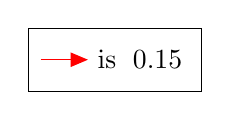
\begin{tikzpicture}
    \node at (0,0) (uses){is};
    \draw[->,red] ([xshift=-0.6cm]uses.west)  -- (uses.west);
    \node at ([xshift=0.4cm]uses.east) {\NeuralNetwork{0.15}};
    \draw[thin] (-1,-0.4) rectangle (1.2,0.4);
  \end{tikzpicture}
}

\begin{frame}{}
%  \myPaper{\footnotesize Ellis, Wong, Nye, ..., Solar-Lezama, Tenenbaum. 2020.}
  \centering
    \only<1>{\vspace{3cm}\hspace*{1cm}\includegraphics[width = 0.3\textwidth]{cycleGraphicalModel0NoGraphical}}
  \only<2>{\vspace{3cm}\hspace*{1cm}\includegraphics[width = 0.3\textwidth]{cycleGraphicalModel1NoGraphical}}
  \only<3>{\includegraphics[width = \textwidth]{cycleGraphicalModel2NoGraphical}}
  \only<4>{\includegraphics[width = \textwidth]{cycleGraphicalModel3NoGraphical}}
  \only<5>{\includegraphics[width = \textwidth]{cycleGraphicalModel4NoGraphical}}
  \only<6>{\includegraphics[width = \textwidth]{cycleGraphicalModel5NoGraphical}}
%  \only<6>{\includegraphics[width = \textwidth]{cycleGraphicalModelAbstraction}}
\end{frame}


\begin{frame}{DreamCoder Domains}
  \Wider[5em]{
    \only<1>{\includegraphics[width = \textwidth]{figures/manyDomainsLarger.png}}%{statement/taskbar2_expended.png}}
%    \only<2>{\includegraphics[width = \textwidth]{figures/manyDomainsSelected.png}}%statement/taskbar2_selected.png}}
  }
\end{frame}

%% \begin{frame}{LOGO Turtle Graphics}
%%   task: given pixels, synthesize graphics program
  
%%   \includegraphics[width = \textwidth]{dc/logoTasks30.png}
  
%% \end{frame}

%% \begin{frame}{LOGO Turtle Graphics -- learning a library}
%%   \Wider[5em]{
%%     \only<1>{\includegraphics[width = \textwidth]{dc/logo_kathy.png}}
%%     \only<2>{\includegraphics[width = \textwidth]{dc/logo_kathy_exploded1.png}}
%%     \only<3>{\includegraphics[width = \textwidth]{dc/logo_kathy_exploded2.png}}
%%     \only<4>{\includegraphics[width = \textwidth]{dc/logo_kathy_exploded3.png}}
%%     \only<5->{\includegraphics[width = \textwidth]{dc/logo_kathy.png}}
      
%%   }

%%   \only<6>{
%%   \messageOverlay{
%%     \begin{tabular}{rl}
%%     circle$(r)$
%%     &\raisebox{-.5\height}{\includegraphics[width = 0.3\textwidth]{dc/logo_primitives/circle_negative.png}}\\
%%     arc$(n,\ell,\theta)$
%%     &\raisebox{-.5\height}{\includegraphics[width = 0.3\textwidth]{../dreamcoder/figures/logo_primitives/arc/arc.png}}
%%   \end{tabular}
%%   }}
%%   \only<5>{
%%     \messageOverlay{\begin{tabular}{c}
%%     radial symmetry$(n,\text{body})$\\
%%     \includegraphics[width = 0.35\textwidth]{dc/rotationalmontage_negative.png}
%%   \end{tabular}}
%%   }
%% %  \myPaper{\small Ellis, Wong, Nye, ..., Solar-Lezama, Tenenbaum. arxiv 2020.}
%% \end{frame}

%% \begin{frame}{What does DreamCoder dream of? (before learning)}
%% %  \emph{before} learning:
%%   \Wider[5em]{
%%     \begin{center}
%%       \includegraphics[height=\textheight]{dc/dreams/beforeLearning36}
%%     \end{center}
%%   }
%% %  \myPaper{Ellis, Wong, Nye, ..., Solar-Lezama, Tenenbaum. 2020.}  
%%   %  \includegraphics[height=3cm]{dc/dreams/cherry_picked/montageSeptember14}    
%% %    \end{tabular}}
%%     %% \only<2>{\begin{tabular}{lll}
%%     %%     before learning&&after learning\\
%%     %%     \includegraphics[width = 0.4\textwidth]{dc/dreams/appendixlogoinitial.png}&&
%%     %%     \includegraphics[width = 0.4\textwidth]{dc/dreams/appendixlogofinal.png}
%%     %%     \end{tabular}}
%% \end{frame}

%% \begin{frame}{What does DreamCoder dream of? (after learning)}
%% %  \emph{after} learning:
%%   \Wider[4em]{
%%     \begin{center}
%%       \includegraphics[height=\textheight]{figures/postDreams6}
%%     \end{center}
%%   }
%% %  \myPaper{Ellis, Wong, Nye, ..., Solar-Lezama, Tenenbaum. 2020.}  

%% %    \end{tabular}}
%%     %% \only<2>{\begin{tabular}{lll}
%%     %%     before learning&&after learning\\
%%     %%     \includegraphics[width = 0.4\textwidth]{dc/dreams/appendixlogoinitial.png}&&
%%     %%     \includegraphics[width = 0.4\textwidth]{dc/dreams/appendixlogofinal.png}
%%     %%     \end{tabular}}
%% \end{frame}

\newcommand{\closex}[2]{
  \renewcommand{\arraystretch}{#1}
  #2
  \renewcommand{\arraystretch}{1}
}
\newcommand{\closey}[2]{
  \setlength{\tabcolsep}{#1}
  #2
  \setlength{\tabcolsep}{6pt}
}

\newcommand{\person}[2]{\closex{0.2}{\begin{tabular}{c}
    {\footnotesize #1}\\
    \includegraphics[width = 1.7cm]{#2}
\end{tabular}}}

%% \begin{frame}{Collaborators}
%% \Wider[6em]{  \centering\begin{tabular}{ccc}
%%   \person{Armando\\{\footnotesize Solar-Lezama}}{collaborators/Armando}&
%%   \person{Josh\\{\footnotesize Tenenbaum}}{collaborators/Josh}&
    
%%     \person{Max Nye}{collaborators/MaxNye}\\
%%     \person{Cathy Wong}{collaborators/cw}&\person{Mathias Sable-Meyer}{collaborators/French}&
%%     \person{Luc Cary}{collaborators/lc}\\
%%     \person{Lucas Morales}{collaborators/Lucas}&\person{Luke Hewitt}{collaborators/lbh}&
%%     \multicolumn{1}{c}{
%%     \begin{tabular}{c}
%%         \textbf{\Large thank}\\
%%         \textbf{\Large you}
%%     \end{tabular}}
%%     \end{tabular}}
  

%% \end{frame}
\end{document}
